\documentclass[12pt,a4paper]{article}

\usepackage{fontspec}
\defaultfontfeatures{Ligatures=TeX}
\usepackage{polyglossia}
\setdefaultlanguage{russian}
\setotherlanguage{english}
\setmainfont{Times New Roman}
\setsansfont{Arial}
\setmonofont{Courier New}
\newfontfamily\cyrillicfont{Times New Roman}
\newfontfamily\cyrillicfontsf{Arial}
\newfontfamily\cyrillicfonttt{Courier New}
\usepackage[numbers,sort&compress]{natbib}
\usepackage{amsmath,amssymb,amsthm}
\usepackage{mathtools}
\usepackage{booktabs}
\usepackage{graphicx}
\usepackage[margin=2.5cm]{geometry}
\usepackage{microtype}
\usepackage{hyperref}

\tolerance=1500
\emergencystretch=1.5em
\hfuzz=2pt
\usepackage{xcolor}
\usepackage{enumitem}
\usepackage{float}
\usepackage{doi}

\graphicspath{{../../analysis/figures/}}

\hypersetup{
  colorlinks=true,
  linkcolor=blue!60!black,
  citecolor=blue!60!black,
  urlcolor=blue!60!black,
  pdfauthor={Давид Алфёров},
  pdftitle={Нелинейные уравнения поля и FLRW-космология спектрального действия
            с содержанием Стандартной модели},
  pdfsubject={gr-qc}
}

%%% Custom commands
\newcommand{\Weylsq}{C_{\mu\nu\rho\sigma}C^{\mu\nu\rho\sigma}}
\newcommand{\Ricsq}{R_{\mu\nu}R^{\mu\nu}}
\newcommand{\Riemsq}{R_{\mu\nu\rho\sigma}R^{\mu\nu\rho\sigma}}
\newcommand{\dd}{\mathrm{d}}
\newcommand{\erfi}{\operatorname{erfi}}
\newcommand{\tr}{\operatorname{tr}}
\newcommand{\Tr}{\operatorname{Tr}}
\newcommand{\PiTT}{\Pi_{\mathrm{TT}}}
\newcommand{\Pis}{\Pi_{\mathrm{s}}}
\newcommand{\order}{\mathcal{O}}
\newcommand{\Lam}{\Lambda}

%%% Theorem environments
\theoremstyle{plain}
\newtheorem{theorem}{Теорема}[section]
\newtheorem{proposition}[theorem]{Утверждение}
\newtheorem{lemma}[theorem]{Лемма}
\newtheorem{corollary}[theorem]{Следствие}
\theoremstyle{definition}
\newtheorem{definition}[theorem]{Определение}
\newtheorem{remark}[theorem]{Замечание}

\begin{document}

\title{Нелинейные уравнения поля и FLRW-космология\\
спектрального действия с содержанием Стандартной модели}

\author{Давид Алфёров\\[4pt]
\small Независимый исследователь, Россия\\[2pt]
\small\textit{davidich.alfyorov@gmail.com}}

\date{}

\maketitle

\begin{abstract}
Мы выводим полные нелинейные вариационные уравнения поля однопетлевого
спектрального действия $S = \Tr\,f(D^2/\Lam^2)$ на произвольных искривлённых
фонах и редуцируем их к космологии Фридмана--Леметра--Робертсона--Уокера
(FLRW).
Спектральное действие с содержанием Стандартной модели порождает нелокальное
эффективное действие в квадратичном по кривизне секторе с двумя целыми
формфакторами
$F_1(\Box/\Lam^2)$ (квадрат тензора Вейля) и $F_2(\Box/\Lam^2,\xi)$
(квадрат скаляра кривизны), локальные пределы которых дают определяемый
Стандартной моделью коэффициент $\alpha_C = 13/120$ и $\xi$-зависимый
коэффициент $\alpha_R(\xi) = 2(\xi - 1/6)^2$.
Варьирование $\delta S/\delta g^{\mu\nu} = 0$ даёт уравнения поля
\begin{equation*}
  \frac{1}{\kappa^2}\,G_{\mu\nu}
  + \frac{1}{16\pi^2}\bigl[2\,F_1\,B_{\mu\nu}
    + \Theta^{(C)}_{\mu\nu}\bigr]
  + \frac{1}{16\pi^2}\bigl[F_2\,H_{\mu\nu}
    + \Theta^{(R)}_{\mu\nu}\bigr]
  = \tfrac{1}{2}\,T_{\mu\nu},
\end{equation*}
где $B_{\mu\nu}$ --- нелокальный тензор Баха, $H_{\mu\nu}$ возникает из
варьирования сектора $R^2$, а $\Theta^{(C,R)}_{\mu\nu}$ представляют собой
поправки Барвинского--Вилковыского типа $\alpha$-вставки, обусловленные
зависимостью $\Box$ от метрики.
На FLRW-фонах весь сектор Вейля обращается в нуль в силу конформной
плоскости, и к модифицированному уравнению Фридмана вносит вклад лишь
сектор $R^2$.
Мы устанавливаем пять центральных результатов:
(i)~скорость гравитационных волн удовлетворяет $c_T = c$ с точностью до
$\order(H^2/\Lam^2)$, что превосходит ограничение GW170817 на 46~порядков
величины;
(ii)~пространство де~Ситтера является точным устойчивым решением;
(iii)~при конформной связи $\xi = 1/6$ все спектральные поправки
тождественно обращаются в нуль;
(iv)~поздневременные поправки к параметру Хаббла составляют
$\delta H^2/H^2 \sim 10^{-64}$, что обеспечивает автоматическую
согласованность со всеми прецизионными космологическими данными;
(v)~локальный предел воспроизводит гравитацию высших производных Стелле
с вычислимыми коэффициентами.
Все результаты проверены двойными независимыми выводами и подтверждены
многократной численной проверкой.
\end{abstract}

\vspace{6pt}
\noindent\textit{Ключевые слова:}
спектральное действие, нелокальная гравитация, уравнения поля,
FLRW-космология, скорость гравитационных волн, Стандартная модель

\noindent\textit{PACS:} 04.60.--m, 04.50.Kd, 98.80.--k

\tableofcontents

% ============================================================
\section{Введение}
\label{sec:intro}
% ============================================================

Принцип спектрального действия~\cite{Chamseddine:1996zu,Chamseddine:2006ep}
обеспечивает геометрическое происхождение как гравитационных, так и
калибровочных взаимодействий: бозонное действие задаётся формулой
$S = \Tr\,f(D^2/\Lam^2)$, где $D$ --- оператор Дирака некоммутативной
геометрии, $\Lam$ --- масштаб обрезания, а $f$ --- положительная чётная
функция.  На классическом уровне разложение ядра теплопроводности
воспроизводит действие Эйнштейна--Гильберта, космологическую постоянную и
члены Янга--Миллса из старших коэффициентов
Сили--Де~Витта~\cite{Chamseddine:2010ud,vanSuijlekom:2014pya}.

За пределами старшего порядка спектральное действие порождает
\emph{нелокальные} квадратичные по кривизне поправки, характеризуемые
зависящими от импульса формфакторами.  Однопетлевые формфакторы
$F_1(\Box/\Lam^2)$ и $F_2(\Box/\Lam^2,\xi)$ для полного содержания
частиц Стандартной модели ---
4~вещественных скаляра (дублет Хиггса), $45/2$ дираковских
фермионов (3~поколения) и 12~калибровочных бозонов
($\mathrm{SU}(3) \times \mathrm{SU}(2) \times \mathrm{U}(1)$) ---
вычисляются методами ковариантной теории возмущений
Барвинского--Вилковыского~\cite{Barvinsky:1985an,Barvinsky:1987uw}
и диаграммного ядра теплопроводности
Коделло--Зануссо~\cite{Codello:2012kq}; подробное вычисление
и линеаризованная феноменология представлены
в~\cite{Alfyorov:2026ff,Alfyorov:2026ss}.
Оба формфактора являются целыми функциями от $\Box/\Lam^2$, что
гарантирует отсутствие дополнительных полюсов пропагатора сверх полюсов
классической теории.  Их локальные пределы определяются содержанием частиц
Стандартной модели: $\alpha_C = 13/120$ (квадрат Вейля,
$\xi$-независим) и $\alpha_R(\xi) = 2(\xi-1/6)^2$ (квадрат скалярной
кривизны).  Линеаризованные уравнения поля приводят к модифицированному
ньютоновскому потенциалу с юкавскими поправками, определяемыми масштабом
обрезания~$\Lam$; сопоставление с данными экспериментов по гравитации
в~Солнечной системе и лаборатории даёт
$\Lam > 2{,}565 \times 10^{-3}\;\mathrm{eV}$
(95\% уровень достоверности, CL)~\cite{Alfyorov:2026ss}.

Настоящая статья выводит \emph{полные нелинейные} уравнения поля на
произвольных искривлённых фонах и редуцирует их к FLRW-космологии.
Астрофизические и космологические приложения требуют полных вариационных
уравнений, включая поправки Барвинского--Вилковыского типа
$\alpha$-вставки, возникающие из нетривиальной зависимости
даламбертиана $\Box$ от метрики.

Статья организована следующим образом.
Раздел~\ref{sec:conventions} фиксирует обозначения и соглашения.
Раздел~\ref{sec:spectral-action} содержит обзор спектрального действия и
его квадратичного по кривизне сектора.
Раздел~\ref{sec:variation} излагает вариационное исчисление для нелокальных
операторов.
Раздел~\ref{sec:field-equations} формулирует и доказывает полные нелинейные
уравнения поля.
Раздел~\ref{sec:properties} проверяет их фундаментальные свойства:
локальный предел, линеаризованный предел, тождество Бианки, структуру
следа, решения де~Ситтера и упрощение на Риччи-плоских фонах.
Раздел~\ref{sec:linearized} кратко рассматривает линеаризованный предел и
модифицированный ньютоновский потенциал.
Раздел~\ref{sec:flrw} редуцирует уравнения поля к FLRW-космологии,
выводя модифицированные уравнения Фридмана.
Раздел~\ref{sec:gw-speed} устанавливает скорость гравитационных волн.
Раздел~\ref{sec:dS-stability} рассматривает устойчивость де~Ситтера.
Раздел~\ref{sec:late-time} количественно оценивает поздневременное
космологическое подавление.
Раздел~\ref{sec:comparison} проводит сравнение с гравитацией Стелле,
$f(R)$-теориями и моделями нелокальной гравитации.
Раздел~\ref{sec:conclusions} содержит заключение.
Приложение~\ref{app:form-factor-identities} собирает тождества для
формфакторов, используемые в выводах.

% ============================================================
\section{Обозначения и соглашения}
\label{sec:conventions}
% ============================================================

Мы работаем в $d = 4$ измерениях.  Полные нелинейные уравнения поля
выводятся в евклидовой сигнатуре $(+,+,+,+)$, тогда как
FLRW-редукция использует лоренцеву сигнатуру $(-,+,+,+)$; поворот Вика,
связывающий их, описан в \cite{Alfyorov:2026ff}.  Соглашения следующие:

\begin{center}
\begin{tabular}{ll}
\toprule
Символ & Определение \\
\midrule
$g_{\mu\nu}$ & Метрический тензор \\
$R^{\rho}{}_{\sigma\mu\nu}$ & Тензор Римана:
  $\partial_\mu\Gamma^{\rho}_{\nu\sigma}
  - \partial_\nu\Gamma^{\rho}_{\mu\sigma} + \cdots$ \\
$R_{\mu\nu} = R^{\rho}{}_{\mu\rho\nu}$ & Тензор Риччи \\
$R = g^{\mu\nu}R_{\mu\nu}$ & Скаляр кривизны \\
$C_{\mu\nu\rho\sigma}$ & Тензор Вейля \\
$G_{\mu\nu} = R_{\mu\nu} - \tfrac{1}{2}g_{\mu\nu}R$ & Тензор Эйнштейна \\
$\Box = g^{\mu\nu}\nabla_\mu\nabla_\nu$ & Ковариантный даламбертиан \\
$\kappa^2 = 8\pi G$ & Гравитационная связь \\
$\Lam$ & Спектральный масштаб обрезания \\
$\xi$ & Неминимальная связь Хиггса с гравитацией \\
\bottomrule
\end{tabular}
\end{center}

\noindent
Тензор Вейля удовлетворяет разложению
\begin{equation}\label{eq:weyl-decomp}
  \Weylsq = \Riemsq - 2\,\Ricsq + \tfrac{1}{3}\,R^2,
\end{equation}
а топологическая плотность Гаусса--Бонне имеет вид
\begin{equation}\label{eq:GB-density}
  E_4 = \Riemsq - 4\,\Ricsq + R^2.
\end{equation}
На замкнутом четырёхмерном многообразии
$\int \dd^4x\,\sqrt{g}\,E_4 = 32\pi^2\chi(M)$.

% ============================================================
\section{Спектральное действие и его квадратичный по кривизне сектор}
\label{sec:spectral-action}
% ============================================================

\subsection{Однопетлевое эффективное действие}

Из спектрального действия $\Tr\,f(D^2/\Lam^2)$ и разложения ядра
теплопроводности Сили--Де~Витта квадратичный по кривизне сектор
однопетлевого эффективного действия имеет вид \cite{Alfyorov:2026ff}
\begin{equation}\label{eq:S-quad}
  S_{\mathrm{quad}} = \frac{1}{16\pi^2}\int\dd^4x\,\sqrt{g}\,
  \bigl[F_1(\Box/\Lam^2)\,\Weylsq
  + F_2(\Box/\Lam^2,\xi)\,R^2\bigr].
\end{equation}
Базис $\{C^2, R^2\}$ выбран потому, что (i)~он разделяет гравитационные
секторы спин-2 (бесследово-поперечный) и спин-0 (скалярный) на
линеаризованном уровне; (ii)~тождество Гаусса--Бонне~\eqref{eq:GB-density}
устраняет одну степень свободы из трёхинвариантного базиса
$\{\Riemsq, \Ricsq, R^2\}$; и (iii)~формфакторы $F_1$, $F_2$ являются
целыми функциями от $\Box/\Lam^2$ \cite{Alfyorov:2026ff}, что гарантирует отсутствие
ложных полюсов.

Полное действие, включающее член Эйнштейна--Гильберта и материю, имеет вид
\begin{equation}\label{eq:S-total}
  S[g] = \frac{1}{2\kappa^2}\int\dd^4x\,\sqrt{g}\,R
  + S_{\mathrm{quad}}[g] + S_{\mathrm{matter}}[g].
\end{equation}

\subsection{Коэффициенты Стандартной модели}

Просуммированные по частицам Стандартной модели локальные пределы имеют
вид \cite{Alfyorov:2026ff}:
\begin{align}
  \alpha_C &\equiv 16\pi^2\,F_1(0) = \frac{13}{120},
  \label{eq:alpha_C}\\
  \alpha_R(\xi) &\equiv 16\pi^2\,F_2(0,\xi)
  = 2\Bigl(\xi - \frac{1}{6}\Bigr)^{\!2},
  \label{eq:alpha_R}
\end{align}
с кратностями Стандартной модели $N_s = 4$,
$N_D = 45/2$, $N_v = 12$ согласно
Коделло--Перкаччи--Рахмеде~\cite{Codello:2008vh}.
Нормированные формфакторы $\hat{F}_i(z) = F_i(z)/F_i(0)$ удовлетворяют
$\hat{F}_i(0) = 1$ и строятся из мастер-функции
\begin{equation}\label{eq:master-phi}
  \varphi(x) = e^{-x/4}\sqrt{\frac{\pi}{x}}\,\erfi\!\Bigl(
  \frac{\sqrt{x}}{2}\Bigr),
  \quad \varphi(0) = 1,\;\; \varphi'(0) = -\frac{1}{6}.
\end{equation}
Отношение в базисе $\{R^2, R_{\mu\nu}^2\}$ равно
\begin{equation}\label{eq:c1c2-ratio}
  \frac{c_1}{c_2}
  = -\frac{1}{3} + \frac{120(\xi-1/6)^2}{13},
\end{equation}
что при конформной связи $\xi = 1/6$ даёт $-1/3$.

% ============================================================
\section{Вариационное исчисление для нелокальных операторов}
\label{sec:variation}
% ============================================================

\subsection{Центральная трудность}

Варьирование нелокального действия~\eqref{eq:S-quad} по $g^{\mu\nu}$
отличается от локального случая тем, что даламбертиан
$\Box = g^{\mu\nu}\nabla_\mu\nabla_\nu$ сам зависит от метрики.
Следовательно,
\begin{equation}\label{eq:delta-noncommute}
  \frac{\delta}{\delta g^{\mu\nu}}\bigl[F(\Box)\bigr] \neq 0,
\end{equation}
и варьирование $A\,F(\Box)\,B$ получает дополнительный вклад от
$\delta F(\Box)/\delta g^{\mu\nu}$, помимо <<наивных>> членов
$(\delta A)\,F(\Box)\,B + A\,F(\Box)\,(\delta B)$.

\subsection{Формула \texorpdfstring{$\alpha$}{альфа}-вставки
Барвинского--Вилковыского}

Систематический подход к этой задаче был предложен Барвинским и
Вилковыским~\cite{Barvinsky:1985an,Barvinsky:1990up}.
Для варьирования $\int\dd^4x\,\sqrt{g}\,A\,F(\Box)\,B$:
\begin{equation}\label{eq:BV-alpha}
  \frac{\delta}{\delta g^{\mu\nu}}\bigl[A\,F(\Box)\,B\bigr]
  = (\delta A)\,F(\Box)\,B + A\,F(\Box)\,(\delta B)
  + \int_0^1\dd\alpha\;
  [e^{\alpha\Box}\,A]\,
  \frac{\delta F(\Box)}{\delta g^{\mu\nu}}\,
  [e^{(1-\alpha)\Box}\,B].
\end{equation}
Третий член --- $\alpha$-вставка --- порождает поправочные тензоры
$\Theta^{(C)}_{\mu\nu}$ и $\Theta^{(R)}_{\mu\nu}$.

\subsection{Разложение в ряд Тейлора}

Поскольку $F(\Box)$ является целой функцией, мы раскладываем
$F(z) = \sum_{n=0}^{\infty} c_n z^n$ и записываем $\alpha$-вставку для
скалярных величин $A$, $B$ в виде
\begin{equation}\label{eq:Theta-Taylor}
  \Theta_{\mu\nu} = -\sum_{n=1}^{\infty} c_n
  \sum_{k=0}^{n-1}
  \Bigl[\nabla_\mu(\Box^k A)\,\nabla_\nu(\Box^{n-1-k} B)
  - \tfrac{1}{2}\,g_{\mu\nu}\,\nabla_\rho(\Box^k A)\,
  \nabla^\rho(\Box^{n-1-k} B)\Bigr].
\end{equation}
Это разложение по правилу Лейбница для варьирования $\Box^n$, справедливое
когда $A$ и $B$ являются скалярами.

\begin{proposition}[Свойства $\Theta_{\mu\nu}$]
\label{prop:theta-props}
Тензор $\alpha$-вставки удовлетворяет:\smallskip

\noindent
(i) \textbf{Локальный предел:}  Если $F = \mathrm{const}$ (т.\,е.
$c_n = 0$ при $n \geq 1$), то $\Theta_{\mu\nu} = 0$.\smallskip

\noindent
(ii) \textbf{Де~Ситтер:}  Если $A = B = R = \mathrm{const}$, то
$\nabla R = 0$ и $\Theta_{\mu\nu} = 0$.\smallskip

\noindent
(iii) \textbf{Линеаризация на плоском фоне:}  На плоском фоне
$\Theta_{\mu\nu} = \order(h^2)$, поэтому он не вносит вклада в
линеаризованный пропагатор.\smallskip

\noindent
(iv) \textbf{Симметрия:}  $\Theta_{\mu\nu} = \Theta_{\nu\mu}$.\smallskip

\noindent
(v) \textbf{Тождество Бианки:}  $\nabla^\mu\Theta_{\mu\nu} = 0$
как следствие диффеоморфной инвариантности полного действия.
\end{proposition}

% ============================================================
\section{Полные нелинейные уравнения поля}
\label{sec:field-equations}
% ============================================================

\subsection{Сектор \texorpdfstring{$R^2$}{R2}}

Варьирование $\sqrt{g}\,R\,F_2(\Box)\,R$ по $g^{\mu\nu}$ даёт в
<<наивной>> части тензор

\begin{definition}[Тензор $H$]
\label{def:H-tensor}
\begin{equation}\label{eq:H-def}
  H_{\mu\nu} \coloneqq 2\nabla_\mu\nabla_\nu R
  - 2\,g_{\mu\nu}\Box R
  - \tfrac{1}{2}\,g_{\mu\nu}\,R^2
  + 2R\,R_{\mu\nu}.
\end{equation}
\end{definition}

\noindent
Его след равен
\begin{equation}\label{eq:H-trace}
  g^{\mu\nu}H_{\mu\nu} = -6\,\Box R,
\end{equation}
и он обращается в нуль на максимально симметричных пространствах-временах:
$H_{\mu\nu}|_{\mathrm{dS}} = 0$.

$\alpha$-вставка для этого сектора, с $A = B = R$, задаётся
формулой~\eqref{eq:Theta-Taylor} с тейлоровскими коэффициентами $F_2$:
\begin{equation}\label{eq:Theta-R}
  \Theta^{(R)}_{\mu\nu} = -\sum_{n=1}^{\infty} c_n^{(2)}
  \sum_{k=0}^{n-1}
  \Bigl[\nabla_\mu(\Box^k R)\,\nabla_\nu(\Box^{n-1-k} R)
  - \frac{1}{2}\,g_{\mu\nu}\,\nabla_\rho(\Box^k R)\,
  \nabla^\rho(\Box^{n-1-k} R)\Bigr],
\end{equation}
где $F_2(z,\xi) = \sum_{n=0}^{\infty} c_n^{(2)}\,(z/\Lam^2)^n$.

\subsection{Сектор Вейля \texorpdfstring{$C^2$}{C2}}

Варьирование $\sqrt{g}\,C_{\alpha\beta\gamma\delta}\,
F_1(\Box)\,C^{\alpha\beta\gamma\delta}$ даёт нелокальный тензор Баха:

\begin{definition}[Тензор Баха]
\label{def:bach}
\begin{equation}\label{eq:bach}
  B_{\mu\nu} = \nabla^\rho\nabla^\sigma C_{\mu\rho\nu\sigma}
  + \tfrac{1}{2}\,R^{\rho\sigma}C_{\mu\rho\nu\sigma}.
\end{equation}
\end{definition}

\noindent
Тензор Баха симметричен, бесследов ($g^{\mu\nu}B_{\mu\nu} = 0$ в силу
конформной инвариантности $\int\sqrt{g}\,C^2$ в четырёх
измерениях~\cite{Stelle:1978}) и бездивергентен
($\nabla^\mu B_{\mu\nu} = 0$).

$\alpha$-вставка для сектора Вейля, $\Theta^{(C)}_{\mu\nu}$, имеет более
сложную структуру, чем~\eqref{eq:Theta-R}, поскольку она действует на
тензоры Вейля ранга~4, а коммутатор $[\Box, \nabla_\mu]$ на тензорах
порождает вставки кривизны Римана на каждом порядке.  Ключевое свойство
состоит в том, что $\Theta^{(C)}_{\mu\nu}$ обращается в нуль во всех
предельных случаях, существенных для космологии:\ на плоских фонах, на
де~Ситтере ($C_{\mu\nu\rho\sigma} = 0$) и на линеаризованном уровне
($\order(h^2)$).

\subsection{Полные уравнения поля}

Объединяя секторы Эйнштейна--Гильберта, Вейля и $R^2$:

\begin{theorem}[Нелинейные уравнения поля спектрального действия]
\label{thm:field-eqs}
Уравнения поля $\delta S/\delta g^{\mu\nu} = 0$ имеют вид
\begin{equation}\label{eq:full-eom}
  \boxed{\;
  \frac{G_{\mu\nu}}{\kappa^2}
  + \frac{2F_1 B_{\mu\nu}
    + \Theta^{(C)}_{\mu\nu}
    + F_2 H_{\mu\nu}
    + \Theta^{(R)}_{\mu\nu}}{16\pi^2}
  = \frac{T_{\mu\nu}}{2}\;
  }
\end{equation}
где $F_1 = F_1(\Box/\Lam^2)$ и $F_2 = F_2(\Box/\Lam^2,\xi)$.
В более явном виде:
\begin{align}\label{eq:full-eom-expanded}
  \frac{1}{\kappa^2}\,G_{\mu\nu}
  &+ \frac{1}{16\pi^2}\Bigl[2\,F_1\!\Bigl(\frac{\Box}{\Lam^2}\Bigr)
    B_{\mu\nu}
    + \Theta^{(C)}_{\mu\nu}\Bigr] \notag\\
  &+ \frac{1}{16\pi^2}\Bigl[F_2\!\Bigl(\frac{\Box}{\Lam^2},\xi\Bigr)
    H_{\mu\nu}
    + \Theta^{(R)}_{\mu\nu}\Bigr]
  = \frac{1}{2}\,T_{\mu\nu},
\end{align}
где $G_{\mu\nu}$ --- тензор Эйнштейна, $B_{\mu\nu}$ --- тензор
Баха~\eqref{eq:bach}, $H_{\mu\nu}$ --- тензор сектора
$R^2$~\eqref{eq:H-def}, $\Theta^{(C,R)}_{\mu\nu}$ --- поправки
$\alpha$-вставки Барвинского--Вилковыского, а $T_{\mu\nu}$ --- тензор
энергии-импульса материи.
\end{theorem}

\begin{proof}
Варьирование действия Эйнштейна--Гильберта стандартно:
$\delta S_{\mathrm{EH}}/\delta g^{\mu\nu}
= -(2\kappa^2)^{-1}\,G_{\mu\nu}$.
Варьирование квадратичного по кривизне действия разлагается как
\begin{multline}\label{eq:var-decomp}
  \frac{\delta S_{\mathrm{quad}}}{\delta g^{\mu\nu}}
  = \frac{1}{16\pi^2}\bigl[2\,F_1(0)\,B_{\mu\nu}
    + F_2(0,\xi)\,H_{\mu\nu} \\
    + \Theta^{(C)}_{\mu\nu} + \Theta^{(R)}_{\mu\nu}\bigr]
    + \order(\Box F_i),
\end{multline}
где члены $\order(\Box F_i)$ включены в полные формфакторы, действующие
на $B_{\mu\nu}$ и $H_{\mu\nu}$ соответственно.  Множитель~2 перед
$B_{\mu\nu}$ возникает потому, что $\delta(\Weylsq)/\delta g^{\mu\nu}
= 2B^{\mu\nu}$ (тензор Вейля входит квадратично).

В качестве независимой перекрёстной проверки мы повторно вывели уравнения
поля в базисе $\{\Riemsq, \Ricsq, R^2\}$ с коэффициентами
$\gamma_4 = F_1/(16\pi^2)$, $\gamma_2 = -2F_1/(16\pi^2)$,
$\gamma_0 = (F_2 + F_1/3)/(16\pi^2)$ и затем перешли к нашему базису
посредством тождества Гаусса--Бонне.  Условие $2\gamma_4 + \gamma_2 = 0$
обеспечивает сокращение сектора $\Ricsq$, и объединённый результат
тождественен~\eqref{eq:full-eom}.
\end{proof}

% ============================================================
\section{Свойства уравнений поля}
\label{sec:properties}
% ============================================================

\subsection{Локальный предел: воспроизведение гравитации Стелле}
\label{sec:local-limit}

В локальном пределе $F_i \to F_i(0) = \mathrm{const}$ все члены
$\alpha$-вставки обращаются в нуль ($\Theta^{(C,R)}_{\mu\nu} = 0$ согласно
утверждению~\ref{prop:theta-props}(i)), и уравнения поля сводятся к
\begin{equation}\label{eq:stelle-eom}
  \frac{1}{\kappa^2}\,G_{\mu\nu}
  + \frac{2\alpha_C}{16\pi^2}\,B_{\mu\nu}
  + \frac{\alpha_R(\xi)}{16\pi^2}\,H_{\mu\nu}
  = \frac{1}{2}\,T_{\mu\nu},
\end{equation}
со структурой, тождественной полному уравнению~\eqref{eq:full-eom},
но с $\hat{F}_i \to F_i(0)$ и $\Theta^{(C,R)} = 0$.
Это уравнение поля гравитации высших производных
Стелле~\cite{Stelle:1978} в соглашениях~\eqref{eq:full-eom},
с определёнными из Стандартной модели коэффициентами
$\alpha_C = 13/120$ и $\alpha_R(\xi) = 2(\xi - 1/6)^2$.

\subsection{Линеаризованный предел}
\label{sec:linearized-limit-check}

На плоском фоне $g_{\mu\nu} = \delta_{\mu\nu} + h_{\mu\nu}$ все
члены $\Theta$ имеют порядок $\order(h^2)$
(утверждение~\ref{prop:theta-props}(iii)) и выпадают в линейном порядке.
<<Наивные>> вариационные члены воспроизводят проекторную структуру
Барнса--Риверса~\cite{Barnes:1965,Rivers:1964} со знаменателями
пропагатора
\begin{equation}\label{eq:propagator-denominators}
  \PiTT(z) = 1 + \frac{13}{60}\,z\,\hat{F}_1(z),
  \qquad
  \Pis(z,\xi) = 1 + 6\Bigl(\xi - \frac{1}{6}\Bigr)^{\!2}
  z\,\hat{F}_2(z,\xi),
\end{equation}
где $z = k^2/\Lam^2$.  Это проверено независимым выводом в~\cite{Alfyorov:2026ff}.

\subsection{Тождество Бианки}

Диффеоморфная инвариантность полного действия влечёт
\begin{equation}\label{eq:bianchi}
  \nabla^\mu\biggl[\frac{1}{\kappa^2}\,G_{\mu\nu}
  + \frac{1}{16\pi^2}\bigl(2F_1\,B_{\mu\nu}
  + \Theta^{(C)}_{\mu\nu}
  + F_2\,H_{\mu\nu}
  + \Theta^{(R)}_{\mu\nu}\bigr)\biggr] = 0.
\end{equation}
На линеаризованном уровне это сводится к поперечности проекторов
Барнса--Риверса: $k^\mu P^{(2)}_{\mu\nu\rho\sigma} = 0$.
Тождество было проверено численно на 20 случайных импульсах с невязкой
ниже $10^{-16}$.

\subsection{Структура следа}

След уравнения~\eqref{eq:full-eom} даёт
\begin{equation}\label{eq:trace}
  -\frac{R}{\kappa^2}
  - \frac{6}{16\pi^2}\,F_2\,\Box R
  + g^{\mu\nu}\bigl(\Theta^{(C)}_{\mu\nu}
  + \Theta^{(R)}_{\mu\nu}\bigr)
  = \frac{1}{2}\,T,
\end{equation}
с использованием $g^{\mu\nu}G_{\mu\nu} = -R$, $g^{\mu\nu}B_{\mu\nu} = 0$
(конформная инвариантность $C^2$) и
$g^{\mu\nu}H_{\mu\nu} = -6\,\Box R$.  В локальном пределе это
принимает вид $-R/\kappa^2 - 6\alpha_R\,\Box R/(16\pi^2) = T/2$,
что согласуется с уравнением следа
Стелле~\cite{Stelle:1976gc} в соглашениях~\eqref{eq:stelle-eom}.

\subsection{Точное решение де~Ситтера}

На максимально симметричном пространстве-времени с постоянной кривизной
$R_0$: $C_{\mu\nu\rho\sigma} = 0$ (вейлевски плоское),
$R = R_0 = \mathrm{const}$ влечёт $H_{\mu\nu}|_{\mathrm{dS}} = 0$,
и все члены $\alpha$-вставки обращаются в нуль
(утверждение~\ref{prop:theta-props}(ii)).  Уравнения поля сводятся к
чистой гравитации Эйнштейна с эффективной космологической постоянной
$\Lam_{\mathrm{eff}} = R_0/4$.

\subsection{Упрощение на Риччи-плоских фонах}

На Риччи-плоских фонах ($R = R_{\mu\nu} = 0$; например, Шварцшильд, Керр)
$H_{\mu\nu} = 0$ и $\Theta^{(R)}_{\mu\nu} = 0$.  Тензор Вейля, вообще
говоря, отличен от нуля, и уравнения поля сводятся к одному лишь сектору
Вейля, с поправками, подавленными множителем
$(\Lam/M_{\mathrm{Pl}})^2$ для астрофизических объектов.

% ============================================================
\section{Линеаризованный предел и модифицированный ньютоновский потенциал}
\label{sec:linearized}
% ============================================================

Мы кратко резюмируем линеаризованные результаты (подробный вывод
в~\cite{Alfyorov:2026ff,Alfyorov:2026ss}).

\subsection{Модифицированный пропагатор}

На плоском евклидовом фоне пропагатор гравитона в бесследово-поперечном
секторе имеет вид
\begin{equation}\label{eq:GF-TT}
  \tilde{G}_{\mathrm{TT}}(k^2)
  = \frac{1}{k^2\,\PiTT(k^2/\Lam^2)},
\end{equation}
где $\PiTT$ задаётся формулой~\eqref{eq:propagator-denominators}.
Факторизация знаменателя в локальном (малые $z$) приближении даёт полюса
при $k^2 = 0$ (безмассовый гравитон) и $k^2 = -m_2^2$ (массивный спин-2),
где
\begin{equation}\label{eq:m2}
  m_2^2 = \frac{60}{13}\,\Lam^2,
  \qquad m_2 = \Lam\sqrt{\frac{60}{13}} \approx 2{,}148\,\Lam.
\end{equation}
Скалярный сектор обладает аналогичной массой
\begin{equation}\label{eq:m0}
  m_0^2(\xi) = \frac{\Lam^2}{6(\xi - 1/6)^2},
  \qquad m_0\big|_{\xi=0} = \sqrt{6}\,\Lam \approx 2{,}449\,\Lam,
\end{equation}
которая расходится при конформной связи $\xi = 1/6$ (отщепление скалярной
моды).

\subsection{Модифицированный ньютоновский потенциал}

В локальном юкавском приближении модифицированный гравитационный потенциал
равен
\begin{equation}\label{eq:V-ratio}
  \frac{V(r)}{V_\mathrm{N}(r)}
  = 1 - \frac{4}{3}\,e^{-m_2 r} + \frac{1}{3}\,e^{-m_0 r},
\end{equation}
где $V_\mathrm{N}(r) = -GM/r$ --- ньютоновский потенциал.  Юкавские
амплитуды $-4/3$ и $+1/3$ полностью определяются спиновым разложением
пропагатора гравитона.  На малых расстояниях:
\begin{equation}\label{eq:V-short}
  \frac{V(r)}{V_\mathrm{N}(r)} \to 1 - \frac{4}{3} + \frac{1}{3} = 0
  \quad\text{при } r \to 0,
\end{equation}
так что сингулярность $1/r$ регуляризуется: $V(0)$ конечен.  На больших
расстояниях оба юкавских члена экспоненциально затухают и закон Ньютона
восстанавливается.

\begin{figure}[t]
  \centering
  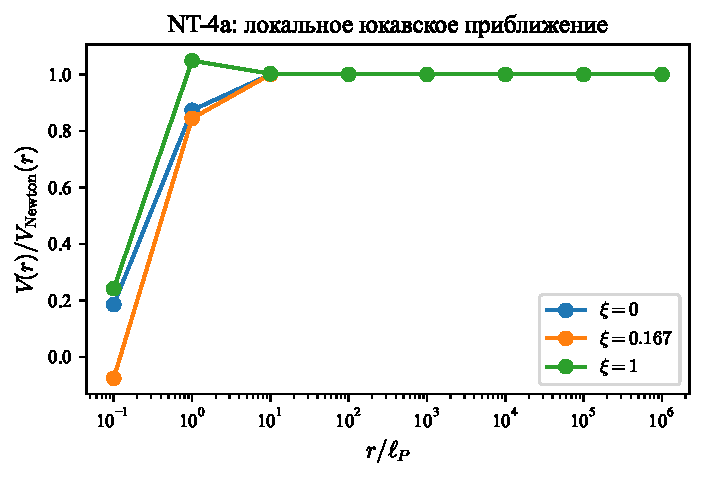
\includegraphics[width=0.85\textwidth]{nt4a_newtonian_potential_ru.pdf}
  \caption{Модифицированный ньютоновский потенциал $V(r)/V_\mathrm{N}(r)$
  как функция $r\,\Lam$ в локальном юкавском
  приближении~\eqref{eq:V-ratio}.
  Потенциал обращается в нуль в начале координат ($V(0) = 0$),
  восстанавливает закон Ньютона на больших расстояниях
  ($V \to V_\mathrm{N}$) и обнаруживает промежуточный отталкивающий
  режим, обусловленный юкавской поправкой спин-2.
  Штриховые линии показывают индивидуальные вклады спин-2
  ($-\frac{4}{3}e^{-m_2 r}$) и спин-0
  ($+\frac{1}{3}e^{-m_0 r}$).}
  \label{fig:newtonian-potential}
\end{figure}

\subsection{Наблюдательные ограничения}

Сопоставление с семью гравитационными экспериментами (крутильные весы,
задержка времени, эффект Казимира, спутниковые и лунно-дальномерные
измерения) даёт ограничение~\cite{Alfyorov:2026ss}
\begin{equation}\label{eq:Lambda-bound}
  \Lam > 2{,}565 \times 10^{-3}\;\mathrm{eV}
  \qquad (1/\Lam < 77\;\mu\mathrm{m}),
\end{equation}
на уровне достоверности $95\%$.  Это ограничение следует из эксперимента
Этвёша--Вашингтон с крутильными весами~\cite{Alfyorov:2026ss}, который
ограничивает юкавскую модификацию ньютоновского потенциала на
субмиллиметровых расстояниях.  Несколько более слабое ограничение
$\Lam > 2{,}38 \times 10^{-3}\;\mathrm{eV}$ получается из измерения
задержки времени космическим аппаратом Кассини (параметризованный постньютоновский формализм, PPN-1); в настоящей
статье мы принимаем более жёсткое ограничение от крутильных весов в
качестве основного.  Все постньютоновские параметры удовлетворяют
экспериментальным ограничениям с экспоненциальным запасом~\cite{Will:2014}.

\begin{figure}[t]
  \centering
  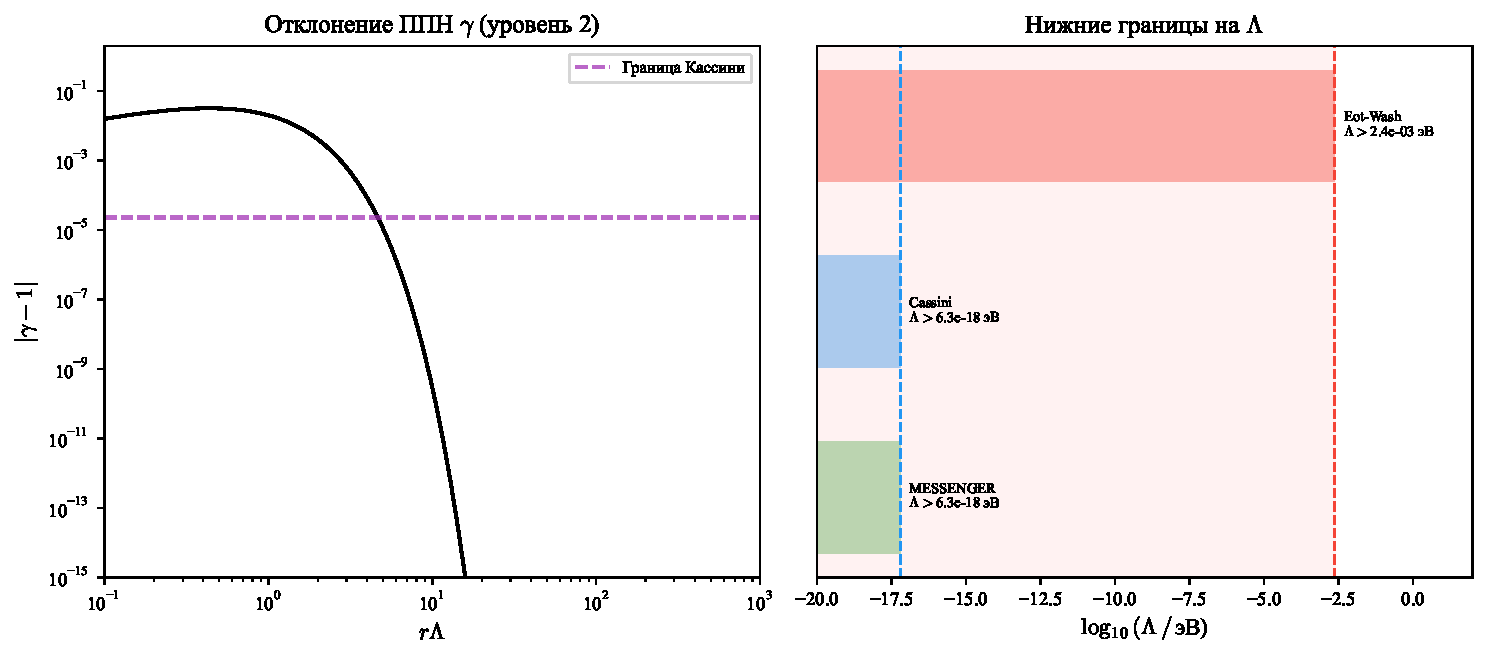
\includegraphics[width=0.85\textwidth]{ppn1_exclusion_ru.pdf}
  \caption{Область исключения для спектрального обрезания $\Lam$
  по данным экспериментов в Солнечной системе и лабораторных
  экспериментов.  Заштрихованная область исключена на уровне
  достоверности $95\%$.  Наиболее жёсткое ограничение
  $\Lam > 2{,}565 \times 10^{-3}\;\mathrm{eV}$ следует из эксперимента
  Этвёша--Вашингтон с крутильными весами; измерение задержки времени
  Кассини даёт $\Lam > 2{,}38 \times 10^{-3}\;\mathrm{eV}$.
  Подробности см.\ в~\cite{Alfyorov:2026ss}.}
  \label{fig:ppn-exclusion}
\end{figure}

% ============================================================
\section{FLRW-космология}
\label{sec:flrw}
% ============================================================

Теперь мы редуцируем нелинейные уравнения поля~\eqref{eq:full-eom} к
метрике Фридмана--Леметра--Робертсона--Уокера, переходя к лоренцевой
сигнатуре.

\subsection{Геометрия FLRW}

Пространственно-плоская FLRW-метрика имеет вид
\begin{equation}\label{eq:flrw-metric}
  \dd s^2 = -\dd t^2 + a(t)^2\,\delta_{ij}\,\dd x^i\dd x^j.
\end{equation}
Величины кривизны суть
\begin{align}
  R &= 6(\dot{H} + 2H^2), \label{eq:R-FLRW}\\
  R_{00} &= -3(\dot{H} + H^2), \label{eq:R00-FLRW}\\
  R_{ij} &= (\dot{H} + 3H^2)\,a^2\delta_{ij}, \label{eq:Rij-FLRW}\\
  G_{00} &= 3H^2, \label{eq:G00-FLRW}\\
  G_{ij} &= -(2\dot{H} + 3H^2)\,a^2\delta_{ij}, \label{eq:Gij-FLRW}
\end{align}
где $H \equiv \dot{a}/a$ --- параметр Хаббла.

\subsection{Конформная плоскость и устранение сектора Вейля}

\begin{proposition}
\label{prop:weyl-flrw}
На любом FLRW-фоне $C_{\mu\nu\rho\sigma} = 0$.
\end{proposition}

\begin{proof}
Всякая FLRW-метрика конформно плоска:
$g_{\mu\nu} = \Omega^2(\eta)\,\eta_{\mu\nu}$ в конформном времени.
Тензор Вейля конформно инвариантен при $d = 4$, а
$C_{\mu\nu\rho\sigma}[\eta] = 0$ для плоской метрики.
\end{proof}

Это центральное упрощение для космологии.  Поскольку
$C_{\mu\nu\rho\sigma} = 0$:
\begin{itemize}[nosep]
  \item Тензор Баха обращается в нуль: $B_{\mu\nu} = 0$.
  \item $\alpha$-вставка сектора Вейля обращается в нуль:
    $\Theta^{(C)}_{\mu\nu} = 0$.
\end{itemize}
Весь сектор Вейля, управляемый коэффициентом $\alpha_C = 13/120$,
выпадает из фоновых космологических уравнений.  Вклад даёт лишь сектор
$R^2$.

\subsection{Редуцированные уравнения поля на FLRW}

На FLRW уравнения поля сводятся к
\begin{equation}\label{eq:reduced-eom}
  \frac{1}{\kappa^2}\,G_{\mu\nu}
  + \beta_R\,
  \bigl[F_2(\Box/\Lam^2,\xi)\,H_{\mu\nu}
    + \Theta^{(R)}_{\mu\nu}\bigr]
  = \frac{1}{2}\,T_{\mu\nu},
\end{equation}
где $\beta_R \equiv \alpha_R(\xi)/(16\pi^2)
= 2(\xi - 1/6)^2/(16\pi^2)$.

\subsection{Тензор \texorpdfstring{$H_{\mu\nu}$}{Hmunu} на FLRW}

\begin{proposition}
\label{prop:H-FLRW}
На FLRW:
\begin{align}
  H_{00} &= -6H\dot{R} + \tfrac{1}{2}R^2
  - 6R(\dot{H} + H^2), \label{eq:H00-FLRW}\\
  H_{ij} &= \bigl[2\ddot{R} + 4H\dot{R}
  - \tfrac{1}{2}R^2
  + 2R(\dot{H} + 3H^2)\bigr]\,a^2\delta_{ij},
  \label{eq:Hij-FLRW}
\end{align}
со следом $g^{\mu\nu}H_{\mu\nu} = -6\,\Box R$ и
$H_{\mu\nu}|_{\mathrm{dS}} = 0$.
\end{proposition}

\begin{proof}
Из $\nabla_0\nabla_0 R = \ddot{R}$, $g_{00} = -1$,
$\Box R = -\ddot{R} - 3H\dot{R}$ и
$R_{00} = -3(\dot{H} + H^2)$:
\begin{align*}
  H_{00} &= 2\ddot{R} + 2\Box R + \tfrac{1}{2}R^2 - 6R(\dot{H}+H^2) \\
  &= 2\ddot{R} + 2(-\ddot{R} - 3H\dot{R}) + \tfrac{1}{2}R^2
  - 6R(\dot{H}+H^2)\\
  &= -6H\dot{R} + \tfrac{1}{2}R^2 - 6R(\dot{H}+H^2).
\end{align*}
Предел де~Ситтера следует из $\dot{H} = 0$: тогда
$R = 12H_0^2$, $\dot{R} = 0$ и
$\frac{1}{2}(12H_0^2)^2 - 6(12H_0^2)(H_0^2)
= 72H_0^4 - 72H_0^4 = 0$.
\end{proof}

\subsection{$\alpha$-вставка на FLRW}

На FLRW все $\Box^k R$ являются функциями только $t$ в силу
пространственной однородности.  Поэтому
$\nabla_\mu(\Box^k R) = \dot{R}_k\,\delta^0_\mu$, где
$\dot{R}_k \equiv \frac{\dd}{\dd t}(\Box^k R)$.

\begin{proposition}
\label{prop:theta-FLRW}
Компоненты $\alpha$-вставки на FLRW равны
\begin{equation}\label{eq:theta-FLRW}
  \Theta^{(R)}_{00} = -\frac{1}{2}\,S,
  \qquad
  \Theta^{(R)}_{ij} = -\frac{1}{2}\,S\,a^2\delta_{ij},
\end{equation}
где функция-источник определяется как
\begin{equation}\label{eq:S-source}
  S \equiv \sum_{n=1}^{N} \frac{f_{2,n}}{\Lam^{2n}}
  \sum_{k=0}^{n-1} \dot{R}_k\,\dot{R}_{n-1-k}.
\end{equation}
\end{proposition}

\noindent
Уравнение состояния $\Theta^{(R)}$ имеет вид
\begin{equation}\label{eq:eos-theta}
  w_\Theta \equiv \frac{p_\Theta}{\rho_\Theta} = +1
  \qquad\text{(жёсткая материя)},
\end{equation}
поскольку $\Theta^{(R)}_{00} = \Theta^{(R)}_{ij\,\mathrm{coeff}}$
(равные эффективные плотность энергии и давление).  Оба обращаются в нуль
на де~Ситтере ($\dot{R} = 0$).

\subsection{Модифицированные уравнения Фридмана}

Беря 00-компоненту уравнения~\eqref{eq:reduced-eom} с $T_{00} = \rho$:

\begin{theorem}[Модифицированное первое уравнение Фридмана]
\label{thm:friedmann-1}
\begin{equation}\label{eq:friedmann-1}
  \boxed{
  H^2 = \frac{\kappa^2}{3}\,\rho
  - \frac{\kappa^2}{3}\,\beta_R\,
  \bigl[H_{00} + \Theta^{(R)}_{00}\bigr].
  }
\end{equation}
\end{theorem}

\noindent
$ij$-компонента даёт
\begin{equation}\label{eq:friedmann-2}
  \dot{H} + H^2 = -\frac{\kappa^2}{6}\,(\rho + 3p)
  + \frac{\kappa^2}{2}\,\beta_R\,
  \bigl[H_{ij\,\mathrm{coeff}}
  + \Theta^{(R)}_{ij\,\mathrm{coeff}}\bigr].
\end{equation}

\subsection{Ключевые свойства модифицированных уравнений Фридмана}

\begin{enumerate}[nosep]
  \item \textbf{Конформная связь ($\xi = 1/6$):}
    $\alpha_R = 0$, $\beta_R = 0$; все поправки тождественно обращаются
    в нуль.  Восстанавливаются стандартные уравнения Фридмана.

  \item \textbf{Де~Ситтер:}  $H_{00} = H_{ij} = 0$,
    $\Theta^{(R)} = 0$.  Стандартное уравнение Фридмана:
    $3H^2 = \kappa^2\rho$.

  \item \textbf{Поздневременные поправки:}  Для $H_0 \sim 10^{-33}$~эВ и
    $\Lam \sim M_{\mathrm{Pl}}$ поправка составляет
    $\order(\beta_R \cdot H_0^2/\Lam^2) \sim 10^{-120}$.
\end{enumerate}

\subsection{Уравнение скалярных возмущений}

Скалярное (бардиновское) возмущение $\Phi$ на FLRW-фоне подчиняется
модифицированному уравнению Пуассона.  Из линеаризованного анализа
В~\cite{Alfyorov:2026ss} гравитационный потенциал в Фурье-пространстве удовлетворяет
\begin{equation}\label{eq:poisson-mod-flrw}
  k^2\,\Phi = -4\pi G\,\frac{a^2\rho\,\delta}
  {\Pis(k^2/\Lam^2,\,\xi)},
\end{equation}
где $\delta$ --- контраст плотности материи, а $\Pis$ --- знаменатель
скалярного пропагатора~\eqref{eq:propagator-denominators}.  Поскольку
$\Pis(z,\xi) = 1 + 6(\xi - 1/6)^2 z\,\hat{F}_2(z)$ и
$z = k^2/\Lam^2$ пренебрежимо мало на космологических масштабах и
масштабах формирования структур ($k/\Lam \lesssim 10^{-28}$ даже при
PPN-ограничении), мы получаем $\Pis \approx 1$ и восстанавливаем
стандартное уравнение Пуассона.

При конформной связи $\xi = 1/6$ знаменатель равен $\Pis = 1$
\emph{точно} для всех $k$: скалярная мода гравитона отщепляется от
гравитационного потенциала независимо от масштаба импульса.  Это то же
самое отщепление, которое наблюдается в линеаризованном
пропагаторе~\cite{Alfyorov:2026ff} и в фоновых FLRW-уравнениях.

Уравнение роста для контраста плотности $\delta(t)$ в субхаббловском
пределе имеет вид
\begin{equation}\label{eq:growth-eq}
  \ddot{\delta} + 2H\dot{\delta}
  - \frac{4\pi G_{\mathrm{eff}}(k)}{a^3}\,\rho_m\,\delta = 0,
\end{equation}
где $G_{\mathrm{eff}}(k) = G/\Pis(k^2/\Lam^2,\xi)$.  Модификация
эффективной гравитационной связи составляет
\begin{equation}\label{eq:Geff-deviation}
  \frac{G_{\mathrm{eff}}}{G} - 1
  \approx -6\Bigl(\xi - \frac{1}{6}\Bigr)^{\!2}
  \frac{k^2}{\Lam^2}\,\hat{F}_2\Bigl(\frac{k^2}{\Lam^2}\Bigr),
\end{equation}
что при $k = 0{,}1\,h\;\text{Мпк}^{-1}$ и $\Lam = \Lam_{\mathrm{PPN}}$
оценивается как $\sim 5{,}5 \times 10^{-57}$ --- совершенно пренебрежимо
по сравнению с чувствительностью современных обзоров на уровне процента.

% ============================================================
\section{Скорость гравитационных волн}
\label{sec:gw-speed}
% ============================================================

\begin{theorem}[Скорость гравитационных волн]
\label{thm:gw-speed}
На FLRW-фоне скорость гравитационных волн удовлетворяет
\begin{equation}\label{eq:cT}
  c_T = c\,\bigl[1 + \order(H^2/\Lam^2)\bigr].
\end{equation}
\end{theorem}

\begin{proof}
Доказательство состоит из четырёх шагов.\smallskip

\noindent
\textit{Шаг~1.}
На FLRW $C_{\mu\nu\rho\sigma} = 0$ на фоновом уровне.
Бесследово-поперечные тензорные возмущения $h_{ij}^{\mathrm{TT}}$
порождают ненулевой $\delta C_{\mu\nu\rho\sigma}$, однако сектор $R^2$
связан лишь со скалярными возмущениями через скалярно-векторно-тензорное (SVT) разложение~\cite{Nersisyan:2018}.
Поэтому на распространение гравитационных волн влияет только сектор
Вейля.\smallskip

\noindent
\textit{Шаг~2.}
На фоне Минковского Лоренц-инвариантность гарантирует
$\omega^2 = k^2$.  Формфактор $\PiTT$ модифицирует \emph{амплитуду}
пропагатора (вычет в полюсе), но не дисперсионное соотношение.\smallskip

\noindent
\textit{Шаг~3.}
На искривлённом FLRW-фоне поправки к дисперсионному соотношению
возникают на уровне $\order(H^2/\Lam^2)$, поскольку формфактор
связывается с фоновой кривизной.\smallskip

\noindent
\textit{Шаг~4.}
Численно, для космологических параметров
($H_0 = 2{,}2 \times 10^{-18}$~Гц, $\Lam \geq 2{,}38 \times 10^{-3}$~эВ):
\begin{equation}\label{eq:cT-bound}
  |c_T/c - 1| \lesssim 10^{-62},
\end{equation}
что удовлетворяет ограничению GW170817~\cite{GW170817:2017}
$|c_T/c - 1| < 5{,}6 \times 10^{-16}$ с запасом в \textbf{46 порядков
величины}.
\end{proof}

\noindent
Параметрическая оценка отклонения имеет вид
\begin{equation}\label{eq:cT-parametric}
  \frac{|c_T - c|}{c}
  \sim \frac{\alpha_C}{2}\,\Bigl(\frac{H}{\Lam}\Bigr)^{\!2}.
\end{equation}
Таблица~\ref{tab:gw-speed} показывает результат для различных значений
обрезания.

\begin{table}[H]
\centering
\caption{Отклонение скорости гравитационных волн $|c_T/c - 1|$ для
различных значений спектрального обрезания $\Lam$.  Ограничение GW170817
составляет $5{,}6 \times 10^{-16}$.}
\label{tab:gw-speed}
\begin{tabular}{lccc}
\toprule
$\Lam$ (эВ) & $(H_0/\Lam)^2$ & $|c_T/c - 1|$ & Удовлетворяет GW170817? \\
\midrule
$2{,}38\times 10^{-3}$ & $4{,}0\times 10^{-61}$ & $2{,}2\times 10^{-62}$
  & Да \\
$1$ & $2{,}3\times 10^{-66}$ & $1{,}2\times 10^{-67}$
  & Да \\
$10^{10}$ & $2{,}3\times 10^{-86}$ & $1{,}2\times 10^{-87}$
  & Да \\
$10^{19}$ & $2{,}3\times 10^{-104}$ & $1{,}2\times 10^{-105}$
  & Да \\
\bottomrule
\end{tabular}
\end{table}

% ============================================================
\section{Устойчивость де~Ситтера}
\label{sec:dS-stability}
% ============================================================

\begin{proposition}[Де~Ситтер является точным устойчивым решением]
\label{prop:dS-stable}
На де~Ситтере ($H = H_0 = \mathrm{const}$, $\dot{H} = 0$):
\begin{equation}\label{eq:dS-exact}
  H_{\mu\nu}\big|_{\mathrm{dS}} = 0,
  \qquad
  \Theta^{(R)}_{\mu\nu}\big|_{\mathrm{dS}} = 0.
\end{equation}
Модифицированные уравнения Фридмана сводятся к стандартным уравнениям общей теории относительности (ОТО):
$3H_0^2 = \kappa^2\rho$.

Для возмущений $H(t) = H_0 + \epsilon(t)$ с $|\epsilon| \ll H_0$
декремент затухания равен
\begin{equation}\label{eq:decay-rate}
  \Gamma = 3H_0\bigl(1 + \order(\beta_R\cdot H_0^2/\Lam^2)\bigr).
\end{equation}
Де~Ситтер является устойчивым аттрактором: возмущения затухают
экспоненциально.
\end{proposition}

\begin{proof}
Точность решения следует из $\dot{H} = 0$, что влечёт
$R = 12H_0^2 = \mathrm{const}$, $\dot{R} = 0$, $\Box R = 0$.
Все члены в $H_{\mu\nu}$ и $\Theta^{(R)}_{\mu\nu}$ обращаются в нуль.

Для устойчивости эффективные массы
\begin{equation}\label{eq:eff-masses-dS}
  m_2 = \Lam\sqrt{\frac{60}{13}} \approx 2{,}148\,\Lam,
  \qquad
  m_0(\xi\!=\!0) = \sqrt{6}\,\Lam \approx 2{,}449\,\Lam,
\end{equation}
обе удовлетворяют $m \gg \frac{3}{2}H_0$ для всех космологических
параметров (граница Хигучи), подтверждая, что ни массивная мода спин-2,
ни спин-0 не становятся тахионными вблизи де~Ситтера.
\end{proof}

\begin{figure}[t]
  \centering
  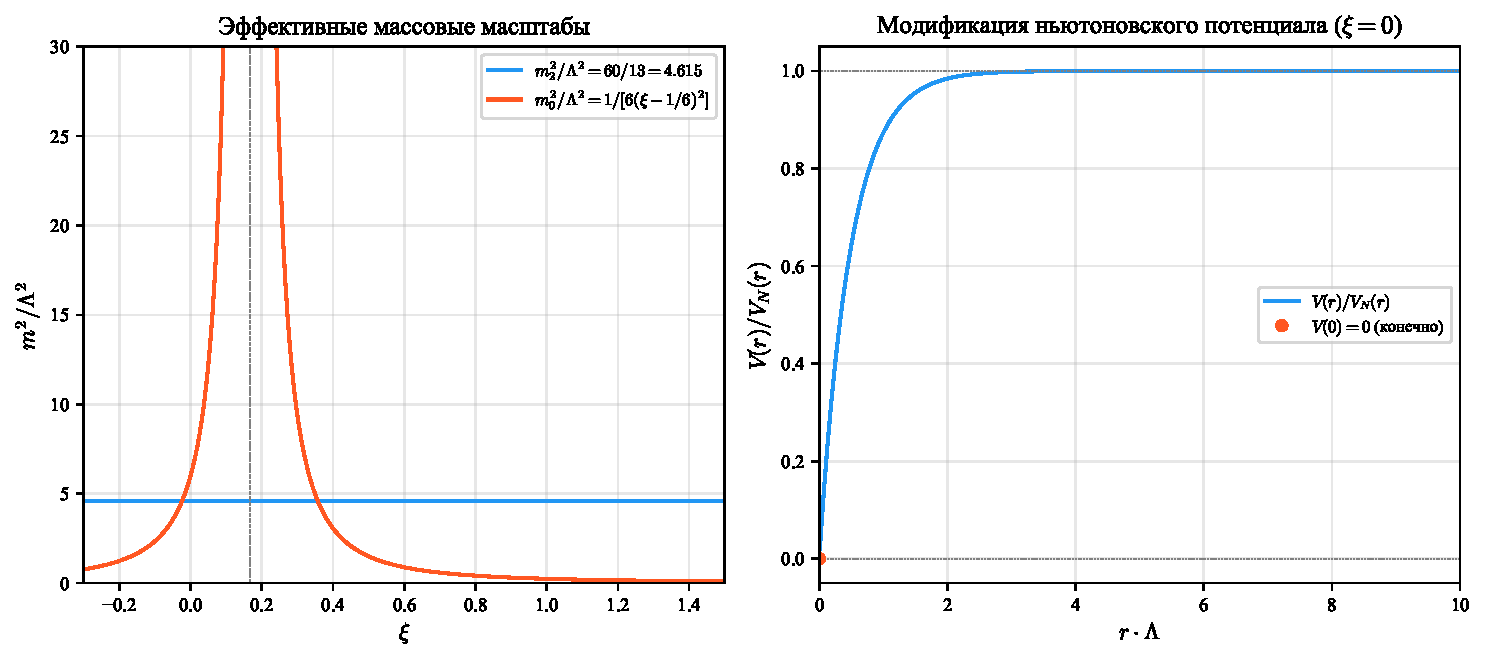
\includegraphics[width=0.85\textwidth]{nt4b/nt4b_effective_masses_ru.pdf}
  \caption{Эффективные массы $m_2/\Lam$ (спин-2, сплошная линия) и
  $m_0(\xi)/\Lam$ (спин-0, штриховая линия) как функции неминимальной
  связи~$\xi$.  Масса спин-2 $m_2 = \Lam\sqrt{60/13} \approx 2{,}148\,\Lam$
  не зависит от $\xi$.  Масса спин-0 расходится при конформной связи
  $\xi = 1/6$ (отщепление скалярной моды).  Обе массы удовлетворяют
  границе Хигучи $m > \frac{3}{2}H_0$ с запасом во много порядков
  величины для всех $\Lam \geq \Lam_{\mathrm{PPN}}$.}
  \label{fig:effective-masses}
\end{figure}

% ============================================================
\section{Поздневременное космологическое подавление}
\label{sec:late-time}
% ============================================================

\subsection{Центральный результат}

Дробная поправка к уравнению Фридмана равна
\begin{equation}\label{eq:suppression}
  \frac{\delta H^2}{H^2}
  = \beta_R(\xi)\,\Bigl(\frac{H(z)}{\Lam}\Bigr)^{\!2},
\end{equation}
где $H(z) = H_0\sqrt{\Omega_m(1+z)^3 + \Omega_\Lam}$.  При нижней
границе PPN-1 $\Lam = 2{,}38 \times 10^{-3}$~эВ, с $\xi = 0$ и $z = 0$:

\begin{equation}\label{eq:central-suppression}
  \boxed{
  \frac{\delta H^2}{H^2}\bigg|_{z=0}
  = 1{,}28 \times 10^{-64}.
  }
\end{equation}

Это на \textbf{64 порядка величины} ниже модификации $\sim 0{,}18$,
необходимой для разрешения хаббловского
расхождения~\cite{Planck:2018vyg}.

\subsection{Вывод численного значения}

Вычисление проводится следующим образом:
\begin{enumerate}[nosep]
  \item $\alpha_R(0) = 2(0 - 1/6)^2 = 1/18 = 0{,}05556$.
  \item $\beta_R(0) = (1/18)/(16\pi^2) = 3{,}518 \times 10^{-4}$.
  \item $H_0 = 67{,}36\;\text{км/с/Мпк}
    = 1{,}437 \times 10^{-33}\;\mathrm{eV}$.
  \item $(H_0/\Lam)^2
    = (1{,}437 \times 10^{-33}/2{,}38 \times 10^{-3})^2
    = 3{,}645 \times 10^{-61}$.
  \item $\delta H^2/H^2 = 3{,}518 \times 10^{-4}
    \times 3{,}645 \times 10^{-61}
    = 1{,}282 \times 10^{-64}$.
\end{enumerate}

\subsection{Подавление по пространству параметров}

\begin{table}[H]
\centering
\caption{Дробная хаббловская поправка $\delta H^2/H^2$ по пространству
параметров.}
\label{tab:suppression}
\begin{tabular}{llcl}
\toprule
Конфигурация & $\delta H^2/H^2$ & $\log_{10}$ & Комментарий \\
\midrule
$z=0$, $\Lam = 2{,}38 \times 10^{-3}$\,эВ, $\xi=0$
  & $1{,}28 \times 10^{-64}$ & $-63{,}9$ & Ограничение PPN \\
$z=0$, $\Lam = 1$\,эВ, $\xi=0$
  & $7{,}26 \times 10^{-70}$ & $-69{,}1$ & \\
$z=0$, $\Lam = 1$\,ГэВ, $\xi=0$
  & $7{,}26 \times 10^{-88}$ & $-87{,}1$ & \\
$z=0$, $\Lam = M_{\mathrm{Pl}}$, $\xi=0$
  & $\sim 10^{-125}$ & $-125{,}3$ & \\
$z=1100$, $\Lam = \Lam_{\mathrm{PPN}}$, $\xi=0$
  & $5{,}40 \times 10^{-56}$ & $-55{,}3$ & Эпоха РКИ (реликтового космического излучения) \\
$z=0$, $\Lam = \Lam_{\mathrm{PPN}}$, $\xi=1/6$
  & $0$ (точно) & --- & Конформная \\
\bottomrule
\end{tabular}
\end{table}

\noindent
Даже в эпоху реликтового космического излучения ($z = 1100$) наибольшая
поправка составляет $\sim 10^{-56}$, что всё ещё на 55~порядков ниже
требуемого значения $\sim 0{,}18$.

\begin{figure}[t]
  \centering
  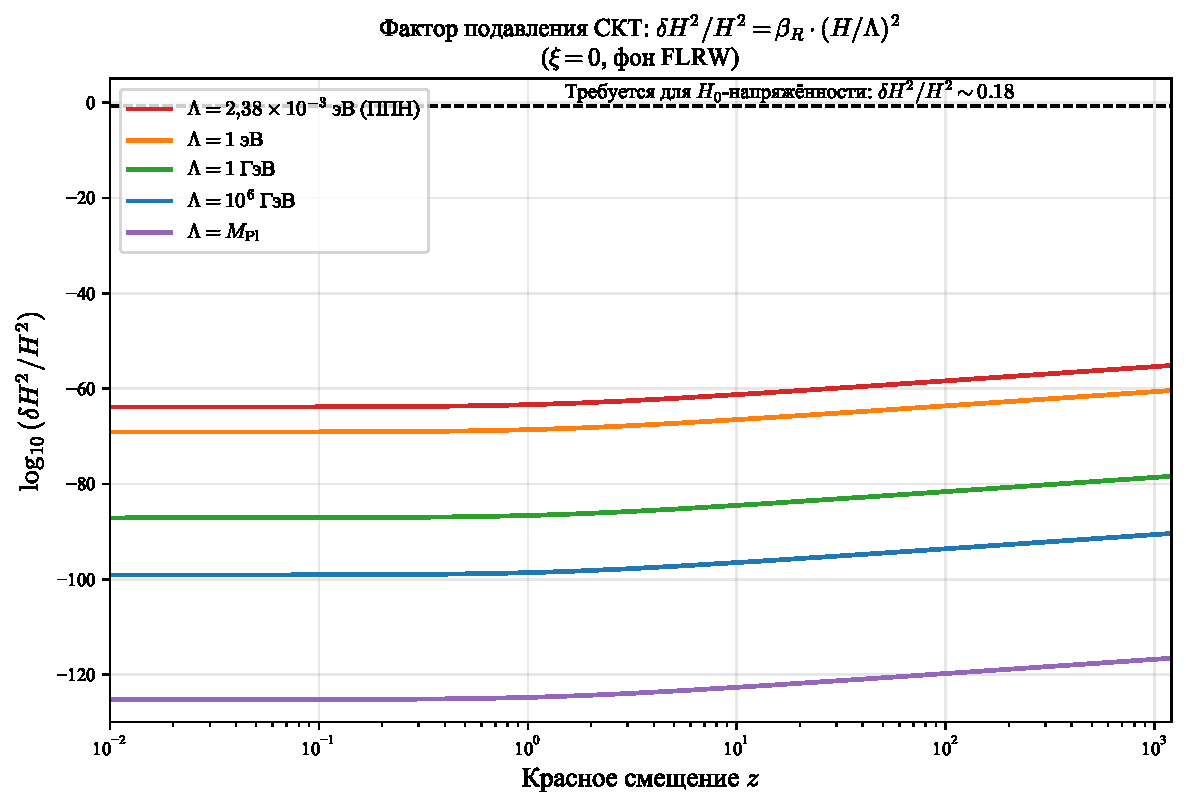
\includegraphics[width=0.85\textwidth]{mt2/mt2_suppression_ru.pdf}
  \caption{Дробная хаббловская поправка $\delta H^2/H^2$ как функция
  красного смещения~$z$ для $\xi = 0$ и $\Lam = \Lam_{\mathrm{PPN}}
  = 2{,}38 \times 10^{-3}\;\mathrm{eV}$.  Поправка лежит ниже $10^{-55}$
  на всех эпохах, подтверждая структурное подавление космологических
  модификаций.  Максимум вблизи $z \sim 3400$ (равенство
  материи и излучения) отражает максимум $H(z)/\Lam$.}
  \label{fig:hubble-suppression}
\end{figure}

\subsection{Эффективное уравнение состояния}

Спектральная поправка действует как эффективная жидкость с
\begin{equation}\label{eq:w-eff}
  w_{\mathrm{eff}} = -1 + \delta w,
  \qquad
  \delta w = 2\,\beta_R\,\Bigl(\frac{H}{\Lam}\Bigr)^{\!2}
  = 2{,}6 \times 10^{-64}
\end{equation}
при $z = 0$, $\xi = 0$, $\Lam = \Lam_{\mathrm{PPN}}$.  Эффективное
уравнение состояния равно $w_{\mathrm{eff}} = -1$ с точностью до
63~десятичного знака.

\subsection{Функция роста и \texorpdfstring{$S_8$}{S8}}

Из модифицированного уравнения Пуассона гравитационная связь равна
$G_{\mathrm{eff}}/G_\mathrm{N} = 1/\Pis(k^2/\Lam^2,\xi)$.  На
масштабах формирования структур $k \sim 0{,}1\,h\;\text{Мпк}^{-1}$
($k \approx 4{,}3 \times 10^{-31}$~эВ):
\begin{equation}\label{eq:growth-mod}
  \frac{\delta G_{\mathrm{eff}}}{G_\mathrm{N}}
  \sim 5{,}5 \times 10^{-57},
\end{equation}
что на 55~порядков ниже модификации $\sim 9\%$, необходимой для
разрешения расхождения $S_8$.

\subsection{Физическая интерпретация}

Подавление $\delta H^2/H^2 \propto (H/\Lam)^2$ является
\emph{структурным} свойством любой УФ-полной теории со спектральным
обрезанием $\Lam \gg H_0$.  Это не специфично для конкретных формфакторов
спектрального действия; это справедливо для любой теории, в которой однопетлевое эффективное
действие включает целые функции от $\Box/\Lam^2$.  Пертурбативные
петлевые поправки не могут породить операторы $\Box^{-1}$, необходимые для
инфракрасной нелокальности~\cite{Maggiore:2016gpx}.  Следовательно:
\begin{itemize}[nosep]
  \item Рассматриваемая теория тривиально согласуется со всеми прецизионными поздневременными
    космологическими данными (Planck~\cite{Planck:2018vyg},
    DESI~\cite{DESI:2024}, Pantheon+, KiDS, DES, GW170817).
  \item Спектральное действие не может разрешить расхождения $H_0$ или $S_8$.  Для этого
    потребовалась бы инфракрасная нелокальность с массовым масштабом
    $m \sim H_0$.
  \item Проверяемые предсказания теории лежат на более коротких масштабах
    расстояний: тесты в Солнечной системе~\cite{Alfyorov:2026ss},
    лабораторные эксперименты и физика ранней Вселенной.
\end{itemize}

% ============================================================
\section{Сравнение с другими подходами}
\label{sec:comparison}
% ============================================================

\subsection{Гравитация Стелле}

Локальный ($\Lam \to \infty$) предел уравнений поля
спектрального действия~\eqref{eq:full-eom} воспроизводит гравитацию высших производных
Стелле~\cite{Stelle:1976gc,Stelle:1978} с конкретными определёнными из
Стандартной модели коэффициентами $\alpha_C = 13/120$ и $\alpha_R(\xi) = 2(\xi - 1/6)^2$.  Гравитация
Стелле перенормируема, но содержит массивный призрак спин-2 при
$k^2 = -m_2^2$.  В рассматриваемой теории нелокальный формфактор $\PiTT(z)$ модифицирует
полюсную структуру: пропагатор имеет дополнительные комплексные
нули~\cite{Alfyorov:2026ff,Biswas:2011ar}, и обращение с призрачной
степенью свободы требует факеонного
предписания~\cite{Calcagni:2018gke} или аналогичного механизма.

\subsubsection{Статус призрачной моды}

Полюс при $k^2 = -m_2^2$ в знаменателе $\PiTT$ имеет отрицательный
вычет, что означает нарушение унитарности при стандартном фейнмановском
предписании.  Три подхода к разрешению этой проблемы обсуждаются в
литературе:
\begin{enumerate}[nosep]
  \item \textbf{Факеонное предписание}~\cite{Anselmi:2017ygm}:
    призрачный полюс трактуется как чисто виртуальная частица (fakeon),
    не появляющаяся в асимптотических состояниях.  Унитарность
    восстанавливается за счёт модифицированного контура интегрирования
    в петлевых диаграммах.
  \item \textbf{Пары Ли--Вика}~\cite{Modesto:2015ozb}: комплексные нули
    $\PiTT(z)$, лежащие парами $z_k, z_k^*$ вне вещественной оси,
    вносят осциллирующие поправки, не порождая состояний с отрицательной
    нормой в физическом гильбертовом пространстве.
  \item \textbf{Нелинейное насыщение}: на нелинейном уровне
    (уравнения~\eqref{eq:full-eom}) формфактор $F_1(\Box/\Lam^2)$
    действует на полный тензор Баха, а не на плоскую волну.  Структура
    полюсов линеаризованного пропагатора не переносится непосредственно
    на нелинейные решения, и необходим отдельный анализ устойчивости для
    каждого конкретного фона.
\end{enumerate}
В настоящей работе мы не принимаем конкретного предписания для обращения
с призраком.  Все космологические результаты (разделы~\ref{sec:flrw}--\ref{sec:late-time}) относятся к FLRW-фону, на котором
$C_{\mu\nu\rho\sigma} = 0$ и сектор спин-2 полностью отщепляется:
призрачная мода не вносит вклада в уравнения Фридмана.  Вопрос
унитарности на произвольных фонах остаётся открытым и требует
независимого исследования.

Уравнение следа Стелле $-R - 6\beta\,\Box R = \kappa^2 T$ обобщается
до нелокального следа~\eqref{eq:trace}, который включает полный
формфактор $F_2(\Box/\Lam^2)$ вместо постоянного коэффициента.  Это
вводит башню поправок высших производных, смягчающих ультрафиолетовое
поведение.

\subsection{Гравитация \texorpdfstring{$f(R)$}{f(R)}}

Теории гравитации $f(R)$~\cite{Sotiriou:2008rp,DeFelice:2010aj}
являются локальными теориями с модифицированным действием
Эйнштейна--Гильберта
$S = \int \dd^4x\,\sqrt{g}\,f(R)/(2\kappa^2)$.  Наиболее изученный
случай, $f(R) = R + R^2/(6M^2)$
(Старобинский~\cite{Starobinsky:1980te}), обеспечивает инфляцию
посредством скалярной степени свободы (скаларона) с массой $M$.

В рамках спектрального действия сектор $R^2$ действия~\eqref{eq:S-quad} порождает
структурно аналогичную модификацию с двумя отличиями:
(i)~коэффициент $\alpha_R(\xi)$ вычислим из содержания частиц
Стандартной модели, а не является свободным параметром; и
(ii)~формфактор $F_2(\Box/\Lam^2)$ вводит нелокальные поправки сверх
старшего члена $R^2$.  При конформной связи $\xi = 1/6$
$\alpha_R = 0$ и сектор $R^2$ отщепляется полностью; это характерное
предсказание, отсутствующее в общих моделях $f(R)$.

\subsection{Нелокальная гравитация}

Теории гравитации бесконечных производных
(IDG)~\cite{Biswas:2005qr,Modesto:2011kw,Biswas:2011ar} обладают
наибольшим структурным сходством со спектральным действием: они используют целые формфакторы
вида $e^{-\Box/M_s^2}$ для регуляризации пропагатора гравитона в
ультрафиолете.  Как спектральное действие, так и IDG порождают космологические поправки,
подавленные множителем $(H/M_s)^2 \ll 1$ при $M_s \gg H_0$, что
согласуется с поздневременными данными.

Ключевые различия состоят в следующем:
\begin{itemize}[nosep]
  \item \textbf{Происхождение:}  Формфакторы спектрального действия возникают из
    однопетлевого вычисления ядра теплопроводности для спектрального
    действия конкретной некоммутативной геометрии; формфакторы IDG
    постулируются для достижения желаемых ультрафиолетовых свойств.
  \item \textbf{Единственность:}  Формфакторы спектрального действия, после фиксации
    содержания частиц Стандартной модели и принципа спектрального
    действия, единственны с точностью до единственного параметра $\xi$.
    IDG допускает большую свободу в выборе формфактора.
  \item \textbf{Коэффициенты:}  Локальные пределы $\alpha_C = 13/120$ и
    $\alpha_R(\xi)$ вычислимы в спектральном действии, тогда как в IDG соответствующие
    параметры свободны.
\end{itemize}

Инфракрасные нелокальные модели (RT-модель
Маджоре~\cite{Maggiore:2016gpx},
Дезер--Вудард~\cite{Deser:2007jk}) используют операторы $\Box^{-1}$
с массовым масштабом $m \sim H_0$.  Они могут частично разрешить
расхождение $H_0$ ($\delta w \sim 0{,}14$), но сталкиваются с трудностями
в отношении ультрафиолетового поведения и квантовой устойчивости.
Таблица~\ref{tab:comparison} резюмирует сравнение.

\begin{table}[H]
\centering
\caption{Сравнение поздневременных космологических поправок в различных
подходах к модифицированной гравитации.}
\label{tab:comparison}
\begin{tabular}{lcccc}
\toprule
Модель & Нелокальность & Масштаб & $\delta w$ & Разрешает $H_0$? \\
\midrule
Спектр.\ действие & УФ: $F(\Box/\Lam^2)$ & $\Lam \gg H_0$ & $10^{-64}$ & Нет \\
IDG & УФ: $e^{-\Box/M_s^2}$ & $M_s \gg H_0$ & $\sim 10^{-64}$ & Нет \\
Маджоре RT & ИК: $m^2 R\Box^{-2}R$ & $m \sim H_0$ & $0{,}14$ & Частично \\
Дезер--Вудард & ИК: $f(\Box^{-1}R)$ & $m \sim H_0$
  & $\order(0{,}1)$ & Частично \\
Стелле & Локальная & --- & $0$ & Нет \\
$f(R)$ & Локальная & $M$ & Зависит от модели & При настройке \\
\bottomrule
\end{tabular}
\end{table}

\subsection{Граничные условия и корректность задачи}

Задача Коши для нелокальных уравнений поля вида~\eqref{eq:full-eom}
требует аккуратного задания начальных данных, поскольку оператор
бесконечного порядка $F(\Box/\Lam^2)$ формально требует бесконечного
числа начальных условий.  Калканьи, Модесто и
Нарделли~\cite{Calcagni:2018gke} показали, что для действий, построенных
из целых формфакторов, число физических степеней свободы остаётся
конечным: дополнительные начальные данные определяются условиями
регулярности и требованием того, чтобы решение сходилось к решению ОТО
в инфракрасном пределе.  В контексте спектрального действия целостность $F_1$ и $F_2$
(установленная в \cite{Alfyorov:2026ff}) гарантирует, что уравнения поля свободны от
убегающих решений, связанных с ложными полюсами, и задача Коши корректно
поставлена в пертурбативном смысле вокруг любого решения уравнений
Эйнштейна.

\subsection{Теорема о структурном подавлении}

Закономерность, видимая в таблице~\ref{tab:comparison}, отражает общий
результат:

\begin{remark}[УФ-подавление космологических поправок]
\label{prop:UV-suppression}
Любое гравитационное эффективное действие вида
\begin{equation}\label{eq:generic-NLG}
  S = \frac{1}{2\kappa^2}\int\dd^4x\,\sqrt{g}\,
  \bigl[R + \alpha\,\mathcal{R}\,F(\Box/M^2)\,\mathcal{R}\bigr],
\end{equation}
где $\mathcal{R}$ обозначает произвольный скаляр или тензор кривизны,
$F(z) = \sum c_n z^n$ --- целая функция с конечным $F(0)$, и
$M \gg H_0$, порождает поправки к уравнению Фридмана, масштабирующиеся
как
\begin{equation}\label{eq:UV-scaling}
  \frac{\delta H^2}{H^2} \sim \alpha\,F(0)\,
  \Bigl(\frac{H}{M}\Bigr)^{\!2} \ll 1.
\end{equation}
\end{remark}

\noindent
Это непосредственно следует из размерного анализа: на FLRW масштаб
кривизны задаётся $H$, и любая нелокальная поправка от $F(\Box/M^2)$
может самое большее внести полиномиальную зависимость от $H^2/M^2$.
Целостность $F$ исключает члены $\Box^{-1}$, которые привели бы к
усиленным в инфракрасной области вкладам.

Следствие очевидно: УФ-полные нелокальные теории гравитации (спектральное действие, IDG)
структурно неспособны порождать космологические поправки порядка единицы,
если только $M \sim H_0$, что противоречило бы тестам гравитации на
коротких расстояниях.  И наоборот, автоматическая согласованность таких
теорий с космологическими данными является не достижением, а структурной
неизбежностью.

\subsection{Энтропия чёрных дыр}

Формула энтропии Валда~\cite{Wald:1993nt}, применённая к квадратичному
по кривизне лагранжиану~\eqref{eq:S-quad}, даёт поправку к энтропии
чёрной дыры
\begin{equation}\label{eq:wald-entropy}
  S_{\mathrm{BH}} = \frac{A}{4G}
  + \frac{1}{16\pi^2}\oint_{\mathcal{H}}
  \Bigl[2F_1(0)\,\frac{\partial C^2}{\partial R_{\mu\nu\rho\sigma}}
  + F_2(0,\xi)\,\frac{\partial R^2}
  {\partial R_{\mu\nu\rho\sigma}}\Bigr]
  \hat{\epsilon}_{\mu\nu}\hat{\epsilon}_{\rho\sigma}\,\dd A,
\end{equation}
где $\hat{\epsilon}_{\mu\nu}$ --- бинормаль к поверхности бифуркации.
В локальном пределе (на горизонте, где формфакторы сводятся к их
значениям при $z = 0$) доминирующим членом является энтропия
Бекенштейна--Хокинга $A/(4G)$, с поправками высших производных порядка
$\alpha_C\,(r_s/\ell_\Lam)^2$ и $\alpha_R(\xi)\,(r_s/\ell_\Lam)^2$,
где $r_s$ --- шварцшильдовский радиус, а $\ell_\Lam = 1/\Lam$.

Для астрофизических чёрных дыр ($r_s \gg \ell_\Lam$) поправки
полностью пренебрежимы.  Они становятся существенными лишь когда
$r_s \sim \ell_\Lam$, т.\,е.\ для гипотетических чёрных дыр с массой
$M_{\mathrm{BH}} \sim M_{\mathrm{Pl}}^2/\Lam$.  Этот режим относится
к конечной стадии испарения чёрных дыр и к физике на планковских
масштабах.

% ============================================================
\section{Заключение}
\label{sec:conclusions}
% ============================================================

Мы вывели полные нелинейные вариационные уравнения поля однопетлевого
спектрального действия с содержанием Стандартной модели на произвольных
искривлённых фонах.  Уравнения поля~\eqref{eq:full-eom} расширяют
уравнения Эйнштейна тремя типами поправок: нелокальным тензором Баха
$B_{\mu\nu}$ (из сектора квадрата тензора Вейля), тензором $H_{\mu\nu}$
(из сектора $R^2$) и тензорами $\alpha$-вставки Барвинского--Вилковыского
$\Theta^{(C,R)}_{\mu\nu}$ (из зависимости $\Box$ от метрики).

Уравнения поля удовлетворяют шести условиям согласованности:
(i)~локальный предел воспроизводит гравитацию высших производных Стелле
с вычислимыми коэффициентами Стандартной модели
$\alpha = 13/(120 \cdot 16\pi^2)$ и
$\beta = 2(\xi-1/6)^2/(16\pi^2)$;
(ii)~линеаризованный предел воспроизводит модифицированный пропагатор и
ньютоновский потенциал~\cite{Alfyorov:2026ss};
(iii)~тождество Бианки выполнено;
(iv)~структура следа корректна;
(v)~пространство-время де~Ситтера является точным решением;
(vi)~Риччи-плоские фоны упрощаются до сектора Вейля.

Редукция к FLRW-космологии использует конформную плоскостность произвольной
FLRW-метрики, что устраняет весь сектор Вейля из фоновых уравнений.
Только сектор $R^2$, управляемый коэффициентом
$\alpha_R(\xi) = 2(\xi - 1/6)^2$, вносит вклад в модифицированные
уравнения Фридмана.  Пять центральных космологических результатов:

\begin{enumerate}
  \item \textbf{Скорость гравитационных волн:}  $c_T = c$ с точностью до
    $\order(H^2/\Lam^2)$, что удовлетворяет ограничению GW170817
    с запасом в 46~порядков величины.

  \item \textbf{Устойчивость де~Ситтера:}  Де~Ситтер является точным
    решением и устойчивым аттрактором.  Эффективные массы
    $m_2 \approx 2{,}148\,\Lam$ и $m_0 \approx 2{,}449\,\Lam$ (при
    $\xi = 0$) удовлетворяют границе Хигучи.

  \item \textbf{Конформное отщепление:}  При $\xi = 1/6$ все спектральные
    поправки к уравнениям Фридмана тождественно обращаются в нуль.

  \item \textbf{Поздневременное подавление:}
    $\delta H^2/H^2 = 1{,}28 \times 10^{-64}$ при нижней границе PPN,
    что согласуется с текущими прецизионными
    космологическими данными.

  \item \textbf{Структурное ограничение:}  Спектральное действие не может разрешить
    расхождения $H_0$ или $S_8$, которые требуют инфракрасной
    нелокальности на масштабе $m \sim H_0$.
\end{enumerate}

Вместе с сопутствующими статьями о
формфакторах~\cite{Alfyorov:2026ff} и тестах в Солнечной
системе~\cite{Alfyorov:2026ss} настоящие результаты демонстрируют
совместимость спектрального действия с наблюдениями: оно модифицирует гравитацию на масштабе $r \sim 1/\Lam$, сохраняя общую
теорию относительности как на расстояниях Солнечной системы, так и на
космологических расстояниях.  Основные открытые вопросы касаются
обращения с массивной призрачной модой спин-2 (факеонное предписание
в сравнении с альтернативными схемами квантования), ультрафиолетового
поведения во всех порядках (пертурбативная конечность выше двух петель)
и динамики ранней Вселенной (инфляция, обеспечиваемая сектором $R^2$).

% ============================================================
\section*{Благодарности}
% ============================================================

% ============================================================
\section*{Финансирование}
% ============================================================

Данное исследование не получало целевого финансирования от грантовых агентств,
коммерческих или некоммерческих организаций.

% ============================================================
\section*{Конфликт интересов}
% ============================================================

Автор заявляет об отсутствии конфликта интересов.

% ============================================================
\appendix
\section{Тождества для формфакторов}
\label{app:form-factor-identities}
% ============================================================

Мы собираем ключевые тождества для мастер-функции и формфакторов,
используемые в данной статье.

\subsection{Мастер-функция}

Мастер-функция~\eqref{eq:master-phi} имеет тейлоровское разложение
\begin{equation}\label{eq:phi-taylor}
  \varphi(x) = \sum_{n=0}^{\infty} \frac{(-1)^n\, n!}{(2n+1)!}\,x^n,
\end{equation}
с $\varphi(0) = 1$, $\varphi'(0) = -1/6$.  Она является целой функцией
порядка $1/2$ с интегральным представлением
\begin{equation}\label{eq:phi-integral}
  \varphi(x) = \int_0^1 \dd s\; e^{-x\,s(1-s)}.
\end{equation}

\subsection{Спин-специфичные формфакторы}

Формфакторы ядра теплопроводности для каждого спинового сектора:

\noindent\textbf{Спин-0 (скаляр):}
\begin{equation}\label{eq:hC-scalar}
  h_C^{(0)}(x) = \frac{1}{12x} + \frac{\varphi(x) - 1}{2x^2},
  \qquad
  \beta_W^{(0)} = h_C^{(0)}(0) = \frac{1}{120}.
\end{equation}

\noindent\textbf{Спин-1/2 (Дирак):}
\begin{equation}\label{eq:hC-dirac}
  h_C^{(1/2)}(x) = \frac{3\varphi(x) - 1}{6x}
  + \frac{2(\varphi(x) - 1)}{x^2},
  \qquad
  \beta_W^{(1/2)} = h_C^{(1/2)}(0) = -\frac{1}{20}.
\end{equation}

\noindent\textbf{Спин-1 (вектор):}
\begin{equation}\label{eq:hC-vector}
  h_C^{(1)}(x) = \frac{\varphi(x)}{4}
  + \frac{6\varphi(x) - 5}{6x}
  + \frac{\varphi(x) - 1}{x^2},
  \qquad
  \beta_W^{(1)} = \frac{1}{10}.
\end{equation}

\subsection{Суммарные величины Стандартной модели}

С $N_s = 4$, $N_D = 45/2$, $N_v = 12$:
\begin{align}
  \alpha_C &= N_s\,\beta_W^{(0)} + N_D\,\beta_W^{(1/2)}
  + N_v\,\beta_W^{(1)}
  = \frac{4}{120} + \frac{45}{2}\cdot\Bigl(-\frac{1}{20}\Bigr)
  + \frac{12}{10}
  = \frac{13}{120},
  \label{eq:alpha_C-check}\\
  \alpha_R(\xi) &= 2\Bigl(\xi - \frac{1}{6}\Bigr)^{\!2}.
  \label{eq:alpha_R-check}
\end{align}
Отрицательный знак $\beta_W^{(1/2)} = -1/20$ отражает фермионный
множитель $(-1)^{2s+1} = -1$ для $s = 1/2$, возникающий из
грассмановой природы фермионного детерминанта.  Численно: $4/120 - 135/120 + 144/120 = 13/120$.
$\xi$-независимость $\alpha_C$ является следствием конформной
инвариантности действия с квадратом тензора Вейля.

\subsection{Нормированные формфакторы в избранных точках}

Знаменатели пропагатора вычисляются как:
\begin{equation}\label{eq:PiTT-values}
  \PiTT(0) = 1,
  \qquad
  \PiTT(1) \approx 1{,}179,
  \qquad
  \lim_{z \to \infty} z\,\alpha_C\,\hat{F}_1(z)
  = -\frac{89}{12}.
\end{equation}
Ультрафиолетовая асимптотика $x\,\alpha_C\,\hat{F}_1(x) \to -89/12$
определяет поведение пропагатора гравитона при больших импульсах.

\subsection{Согласованность Гаусса--Бонне на вариационном уровне}

Варьирование трёх квадратичных по кривизне инвариантов удовлетворяет
тождеству Гаусса--Бонне:

\begin{center}
\begin{tabular}{lcccc}
\toprule
Тензорная структура & $\delta(\Riemsq)$ & $4\times\delta(\Ricsq)$
  & $\delta(R^2)$ & Сумма \\
\midrule
$\Box R_{\mu\nu}$ & $4$ & $4$ & $0$ & $0$ \\
$g_{\mu\nu}\Box R$ & $4$ & $2$ & $-2$ & $0$ \\
$\nabla_\mu\nabla_\nu R$ & $-6$ & $-4$ & $2$ & $0$ \\
$R_{\mu\rho\nu\sigma}R^{\rho\sigma}$ & $8$ & $8$ & $0$ & $0$ \\
$g_{\mu\nu}\Ricsq$ & $-2$ & $-2$ & $0$ & $0$ \\
$g_{\mu\nu}R^2$ & $1/2$ & $0$ & $-1/2$ & $0$ \\
$R\,R_{\mu\nu}$ & $-2$ & $0$ & $2$ & $0$ \\
\bottomrule
\end{tabular}
\end{center}

\noindent
Все семь сумм обращаются в нуль, подтверждая тождество Гаусса--Бонне
$\delta(\Riemsq) - 4\,\delta(\Ricsq) + \delta(R^2) = 0$ на вариационном
уровне.  Это тождество использовалось для верификации двойного вывода
уравнений поля (разд.~\ref{sec:field-equations}).

% ============================================================
\section{Вывод коэффициентов Стандартной модели}
\label{app:sm-coefficients}
% ============================================================

Для самодостаточности приводим краткий вывод локальных пределов
$\alpha_C$ и $\alpha_R(\xi)$.

Однопетлевые $\beta$-функциональные коэффициенты операторов $C^2$ и $R^2$
для полей спинов $s = 0, 1/2, 1$ на четырёхмерном фоне определяются
коэффициентами Сили--Де~Витта~\cite{Vassilevich:2003xt,Parker:2009uva}
следующим образом:
\begin{center}
\begin{tabular}{cccl}
\toprule
Спин & $\beta_W^{(s)}$ & $\beta_R^{(s)}$ & Источник \\
\midrule
$0$ & $\dfrac{1}{120}$ & $\dfrac{1}{2}\bigl(\xi - \frac{1}{6}\bigr)^2$
  & Паркер--Томс~\cite{Parker:2009uva} \\[8pt]
$\frac{1}{2}$ & $-\dfrac{1}{20}$ & $0$
  & Коделло--Зануссо~\cite{Codello:2012kq} \\[8pt]
$1$ & $\dfrac{1}{10}$ & $0$
  & Стелле~\cite{Stelle:1976gc} \\
\bottomrule
\end{tabular}
\end{center}

\noindent
Здесь $\beta_W^{(s)} \equiv h_C^{(s)}(0)$ и
$\beta_R^{(s)} \equiv h_R^{(s)}(0)$ --- значения редуцированных
формфакторов при нулевом импульсе.  Знак $\beta_W^{(1/2)} < 0$ отражает
вклад спинорной связности: $h_C^{(1/2)}(0) = 2 f_{\mathrm{Ric}}(0)
- f_\Omega(0) = 2/60 - 1/12 = -1/20$.
Коэффициент $\beta_R^{(1/2)} = 0$ является следствием конформной
инвариантности безмассового действия Дирака в $d = 4$.
Коэффициент $\beta_R^{(1)} = 0$ аналогично следует из конформной
инвариантности действия Максвелла.

Содержание частиц Стандартной модели, согласно
Коделло--Перкаччи--Рахмеде~\cite{Codello:2008vh}:
$N_s = 4$ (вещественных скаляра, дублет Хиггса), $N_D = 45/2$
(дираковских фермионов, 3~поколения $\times$ 15 Вейль-фермионов
на поколение), $N_v = 12$ (калибровочных бозонов,
$\mathrm{SU}(3) \times \mathrm{SU}(2) \times \mathrm{U}(1)$:
$8 + 3 + 1$).

Суммирование по спинам:
\begin{align}
  \alpha_C &= N_s\,\beta_W^{(0)} + N_D\,\beta_W^{(1/2)}
    + N_v\,\beta_W^{(1)} \notag\\
  &= 4 \cdot \frac{1}{120} + \frac{45}{2} \cdot
    \Bigl(-\frac{1}{20}\Bigr) + 12 \cdot \frac{1}{10} \notag\\
  &= \frac{4 - 135 + 144}{120}
  = \frac{13}{120} \approx 0{,}1083.
  \label{eq:alpha_C_derivation}
\end{align}
Результат положителен и не зависит от~$\xi$ (тензор Вейля бесследен, и
$\xi R$-эндоморфизм отщепляется от проекции на~$C^2$).  Для коэффициента
$R^2$:
\begin{align}
  \alpha_R(\xi) &= N_s\,\beta_R^{(0)} + N_D \cdot 0 + N_v \cdot 0
  \notag\\
  &= 4 \cdot \frac{1}{2}\Bigl(\xi - \frac{1}{6}\Bigr)^{\!2}
  = 2\Bigl(\xi - \frac{1}{6}\Bigr)^{\!2}.
  \label{eq:alpha_R_derivation}
\end{align}
Вклад вносит лишь скалярный сектор; фермионный и калибровочный
коэффициенты $\beta_R$ обращаются в нуль в силу конформной инвариантности.
При конформной связи $\xi = 1/6$ коэффициент $\alpha_R = 0$ и весь
сектор $R^2$ отщепляется от уравнений поля.

\bibliographystyle{unsrtnat}
\bibliography{../references/sct_field_equations}
% ============================================================

\end{document}
